\chapter{Manipulación de bits}

Todos los datos en los programas de computadora se almacenan internamente como bits,
es decir, como números 0 y 1.
Este capítulo discute la representación de bits
de los enteros y muestra ejemplos
de cómo usar operaciones de bits.
Resulta que hay muchos usos para
la manipulación de bits en la programación de algoritmos.

\section{Representación de bits}

\index{representación de bits}

En la programación, un entero de $n$ bits se guarda internamente
como un número binario que consta de $n$ bits.
Por ejemplo, el tipo \texttt{int} en C++ es
un tipo de 32 bits, lo que significa que cada número \texttt{int}
consta de 32 bits.

Aquí está la representación de bits del
número \texttt{int} 43:
\[00000000000000000000000000101011\]
Los bits en la representación se indexan de derecha a izquierda.
Para convertir una representación de bits $b_k \cdots b_2 b_1 b_0$ en un número,
podemos usar la fórmula
\[b_k 2^k + \ldots + b_2 2^2 + b_1 2^1 + b_0 2^0.\]
Por ejemplo,
\[1 \cdot 2^5 + 1 \cdot 2^3 + 1 \cdot 2^1 + 1 \cdot 2^0 = 43.\]

La representación de bits de un número es
\key{con signo} o \key{sin signo}.
Por lo general, se utiliza una representación con signo,
lo que significa que se pueden representar
números negativos y positivos.
Una variable con signo de $n$ bits puede contener cualquier
entero entre $-2^{n-1}$ y $2^{n-1}-1$.
Por ejemplo, el tipo \texttt{int} en C++ es
un tipo con signo, por lo que una variable \texttt{int} puede contener cualquier
entero entre $-2^{31}$ y $2^{31}-1$.

El primer bit en una representación con signo
es el signo del número (0 para números no negativos
y 1 para números negativos) y
los $n-1$ bits restantes contienen la magnitud del número.
Se utiliza el \key{complemento a dos}, lo que significa que el
número opuesto de un número se calcula primero
invirtiendo todos los bits en el número,
y luego incrementando el número en uno.

Por ejemplo, la representación de bits del
número \texttt{int} $-43$ es
\[11111111111111111111111111010101.\]

En una representación sin signo, solo se pueden usar
números no negativos, pero el límite superior para los valores es el doble.
Una variable sin signo de $n$ bits puede contener cualquier
entero entre $0$ y $2^n-1$.
Por ejemplo, en C++, una variable \texttt{unsigned int}
puede contener cualquier entero entre $0$ y $2^{32}-1$.

Existe una conexión entre las
representaciones:
un número con signo $-x$ es igual a un número sin signo $2^n-x$.
Por ejemplo, el siguiente código muestra que
el número con signo $x=-43$ es igual al número sin signo
$y=2^{32}-43$:
\begin{lstlisting}
int x = -43;
unsigned int y = x;
cout << x << "\n"; // -43
cout << y << "\n"; // 4294967253
\end{lstlisting}

Si un número es mayor que el límite superior
de la representación de bits, el número se desbordará.
En una representación con signo,
el siguiente número después de $2^{n-1}-1$ es $-2^{n-1}$,
y en una representación sin signo,
el siguiente número después de $2^n-1$ es $0$.
Por ejemplo, considera el siguiente código:
\begin{lstlisting}
int x = 2147483647
cout << x << "\n"; // 2147483647
x++;
cout << x << "\n"; // -2147483648
\end{lstlisting}

Inicialmente, el valor de $x$ es $2^{31}-1$.
Este es el valor más grande que se puede almacenar
en una variable \texttt{int},
por lo que al incrementarse se desborda hacia $-2^{31}$.


\section{Operaciones de bits}

\newcommand\XOR{\mathbin{\char`\^}}

\subsubsection{Operación and}

\index{and (operación)}

La operación \key{and} $x$ \& $y$ produce un número
que tiene bits uno en las posiciones donde ambos
$x$ e $y$ tienen bits uno.
Por ejemplo, $22$ \& $26$ = 18, porque

\begin{center}
    \begin{tabular}{rrr}
           & 10110 & (22) \\
        \& & 11010 & (26) \\
        \hline
        =  & 10010 & (18) \\
    \end{tabular}
\end{center}

Usando la operación and, podemos verificar si un número
$x$ es par porque
$x$ \& $1$ = 0 si $x$ es par, y
$x$ \& $1$ = 1 si $x$ es impar.
Más generalmente, $x$ es divisible por $2^k$
exactamente cuando $x$ \& $(2^k-1)$ = 0.

\subsubsection{Operación or}

\index{or (operación)}

La operación \key{or} $x$ | $y$ produce un número
que tiene bits uno en posiciones donde al menos uno
de $x$ e $y$ tienen bits uno.
Por ejemplo, $22$ | $26$ = 30, porque


\begin{center}
    \begin{tabular}{rrr}
               & 10110 & (22) \\
        $\XOR$ & 11010 & (26) \\
        \hline
        =      & 01100 & (12) \\
    \end{tabular}
\end{center}

\subsubsection{Operación not}

\index{not (operación)}

La operación \key{not} \textasciitilde$x$
produce un número donde todos los bits de $x$
han sido invertidos.
La fórmula \textasciitilde$x = -x-1$ se mantiene,
por ejemplo, \textasciitilde$29 = -30$.

El resultado de la operación not a nivel de bit
depende de la longitud de la representación de bits,
porque la operación invierte todos los bits.
Por ejemplo, si los números son de 32 bits,
números \texttt{int}, el resultado es el siguiente:

\begin{center}
    \begin{tabular}{rrrr}
        $x$                & = & 00000000000000000000000000011101 & (29)    \\
        \textasciitilde$x$ & = & 11111111111111111111111111100010 & $(-30)$ \\
    \end{tabular}
\end{center}

\subsubsection{Desplazamiento de bits}

\index{desplazamiento de bits}

El desplazamiento de bits a la izquierda $x < < k$ añade $k$
bits de cero al número,
y el desplazamiento de bits a la derecha $x > > k$
elimina los últimos $k$ bits del número.
Por ejemplo, $14 < < 2 = 56$,
porque $14$ y $56$ corresponden a 1110 y 111000.
De manera similar, $49 > > 3 = 6$,
porque $49$ y $6$ corresponden a 110001 y 110.

Ten en cuenta que $x < < k$
corresponde a multiplicar $x$ por $2^k$,
y $x > > k$
corresponde a dividir $x$ por $2^k$
redondeado hacia abajo a un entero.

\subsubsection{Aplicaciones}

Un número de la forma $1 < < k$ tiene un bit de uno
en la posición $k$ y todos los demás bits son cero,
por lo que podemos usar tales números para acceder a bits individuales de los números.
En particular, el bit $k$ de un número es uno
exactamente cuando $x$ \& $(1 < < k)$ no es cero.
El siguiente código imprime la representación de bits
de un número \texttt{int} $x$:

\begin{lstlisting}
for (int i = 31; i >= 0; i--) {
    if (x & (1 << i)) cout << "1";
    else cout << "0";
}
\end{lstlisting}

También es posible modificar bits individuales
de números usando ideas similares.
Por ejemplo, la fórmula $x$ | $(1 < < k)$
establece el bit $k$ de $x$ en uno,
la fórmula
$x$ \& \textasciitilde $(1 < < k)$
establece el bit $k$ de $x$ en cero,
y la fórmula
$x$ $\XOR$ $(1 < < k)$
invierte el bit $k$ de $x$.

La fórmula $x$ \& $(x-1)$ establece el último
bit uno de $x$ a cero,
y la fórmula $x$\nobreakspace\&\nobreakspace$-x$ establece todos los
bits uno a cero, excepto el último bit uno.
La fórmula $x$\nobreakspace|\nobreakspace$(x-1)$
invierte todos los bits después del último bit uno.
Además, se debe tener en cuenta que un número positivo $x$ es
una potencia de dos exactamente cuando $x$\nobreakspace\&\nobreakspace$(x-1) = 0$.

\subsubsection*{Funciones adicionales}

El compilador g++ proporciona las siguientes
funciones para contar bits:

\begin{itemize}[itemsep=0em,topsep=0.5em]
    \item $\texttt{\_\_builtin\_clz}(x)$:
          la cantidad de ceros al principio del número
    \item $\texttt{\_\_builtin\_ctz}(x)$:
          la cantidad de ceros al final del número
    \item $\texttt{\_\_builtin\_popcount}(x)$:
          la cantidad de unos en el número
    \item $\texttt{\_\_builtin\_parity}(x)$:
          la paridad (par o impar) de la cantidad de unos
\end{itemize}

\noindent
Las funciones se pueden utilizar de la siguiente manera:
\begin{lstlisting}
int x = 5328; // 00000000000000000001010011010000
cout << __builtin_clz(x) << "\n"; // 19
cout << __builtin_ctz(x) << "\n"; // 4
cout << __builtin_popcount(x) << "\n"; // 5
cout << __builtin_parity(x) << "\n"; // 1
\end{lstlisting}

\section{Representación de conjuntos}

Cada subconjunto de un conjunto
$\{0,1,2,\ldots,n-1\}$
se puede representar como un número entero de $n$ bits
cuyos bits unos indican qué
elementos pertenecen al subconjunto.
Esta es una forma eficiente de representar conjuntos,
porque cada elemento requiere solo un bit de memoria,
y las operaciones de conjuntos se pueden implementar como operaciones de bits.

Por ejemplo, dado que \texttt{int} es un tipo de 32 bits,
un número \texttt{int} puede representar cualquier subconjunto
del conjunto $\{0,1,2,\ldots,31\}$.
La representación de bits del conjunto $\{1,3,4,8\}$ es
\[00000000000000000000000100011010,\]
que corresponde al número $2^8+2^4+2^3+2^1=282$.

\subsubsection{Implementación de conjuntos}

El siguiente código declara una variable \texttt{int}
$x$ que contiene el subconjunto $\{1,3,4,8\}$ del
conjunto $\{0,\ldots,31\}$, y luego imprime el tamaño del conjunto.
\begin{lstlisting}
int x = 0;
x |= (1 << 1);
x |= (1 << 3);
x |= (1 << 4);
x |= (1 << 8);
cout << __builtin_popcount(x) << "\n"; // 4
\end{lstlisting}
El siguiente código imprime todos
los elementos que pertenecen al conjunto:
\begin{lstlisting}
for (int i = 0; i < 32; i++) {
    if (x & (1 << i)) cout << i << " ";
}
// 1 3 4 8
\end{lstlisting}

\subsubsection{Operaciones de conjuntos}

Las operaciones de conjuntos se pueden implementar como operaciones de bits de la siguiente manera:

\begin{center}
    \begin{tabular}{lll}
                     & sintaxis de conjuntos & sintaxis de bits            \\
        \hline
        intersección & $a \cap b$            & $a$ \& $b$                  \\
        unión        & $a \cup b$            & $a$ | $b$                   \\
        complemento  & $\bar a$              & \textasciitilde$a$          \\
        diferencia   & $a \setminus b$       & $a$ \& (\textasciitilde$b$) \\
    \end{tabular}
\end{center}

Por ejemplo, el siguiente código primero construye
los conjuntos $x=\{1,3,4,8\}$ e $y=\{3,6,8,9\}$,
y luego construye el conjunto $z = x \cup y = \{1,3,4,6,8,9\}$:

\begin{lstlisting}
int x = (1 << 1) | (1 << 3) | (1 << 4) | (1 << 8);
int y = (1 << 3) | (1 << 6) | (1 << 8) | (1 << 9);
int z = x | y;
cout << __builtin_popcount(z) << "\n"; // 6
\end{lstlisting}

\subsubsection{Iteración a través de subconjuntos}

El siguiente código recorre
los subconjuntos de $\{0,1,\ldots,n-1\}$:

\begin{lstlisting}
for (int b = 0; b < (1 << n); b++) {
    // procesar subconjunto b
}
\end{lstlisting}
El siguiente código recorre
los subconjuntos con exactamente $k$ elementos:
\begin{lstlisting}
for (int b = 0; b < (1 << n); b++) {
    if (__builtin_popcount(b) == k) {
        // procesar subconjunto b
    }
}
\end{lstlisting}
El siguiente código recorre los subconjuntos
de un conjunto $x$:
\begin{lstlisting}
int b = 0;
do {
    // procesar subconjunto b
} while (b = (b - x) & x);
\end{lstlisting}

\section{Optimizaciones de bits}

Muchos algoritmos se pueden optimizar utilizando
operaciones de bits.
Estas optimizaciones no cambian la
complejidad del tiempo del algoritmo,
pero pueden tener un gran impacto
en el tiempo de ejecución real del código.
En esta sección discutimos ejemplos
de tales situaciones.

\subsubsection{Distancias de Hamming}

\index{distancia de Hamming}
La \key{distancia de Hamming}
$\texttt{hamming}(a,b)$ entre dos
cadenas $a$ y $b$ de igual longitud es
el número de posiciones en las que las cadenas difieren.
Por ejemplo,
\[\texttt{hamming}(01101,11001)=2.\]

Considera el siguiente problema: dada
una lista de $n$ cadenas de bits, cada una de longitud $k$,
calcula la distancia mínima de Hamming
entre dos cadenas en la lista.
Por ejemplo, la respuesta para $[00111,01101,11110]$
es 2, porque
\begin{itemize}[noitemsep]
    \item $\texttt{hamming}(00111,01101)=2$,
    \item $\texttt{hamming}(00111,11110)=3$, y
    \item $\texttt{hamming}(01101,11110)=3$.
\end{itemize}

Una forma directa de resolver el problema es
recorrer todos los pares de cadenas y calcular
sus distancias de Hamming,
lo que produce un algoritmo de tiempo $O(n^2 k)$.
La siguiente función se puede utilizar para
calcular distancias:
\begin{lstlisting}
int hamming(string a, string b) {
    int d = 0;
    for (int i = 0; i < k; i++) if (a[i] != b[i]) d++;
    return d;
}
\end{lstlisting}

Sin embargo, si $k$ es pequeño, podemos optimizar el código
almacenando las cadenas de bits como enteros y
calculando las distancias de Hamming usando operaciones de bits.
En particular, si $k \le 32$, podemos almacenar
las cadenas como valores \texttt{int} y usar la
siguiente función para calcular distancias:
\begin{lstlisting}
int hamming(int a, int b) {
    return __builtin_popcount(a ^ b);
}
\end{lstlisting}
En la función anterior, la operación xor construye
una cadena de bits que tiene unos en posiciones
donde $a$ y $b$ difieren.
Luego, se calcula el número de bits usando
la función \texttt{\_\_builtin\_popcount}.

Para comparar las implementaciones, generamos
una lista de 10.000 cadenas de bits aleatorias de longitud 30.
Usando el primer enfoque, la búsqueda tomó
13,5 segundos, y después de la optimización de bits,
sólo tomó 0,5 segundos.
Por lo tanto, el código optimizado de bits fue casi
30 veces más rápido que el código original.

\subsubsection{Contando subcuadrículas}

Como otro ejemplo, considera el
siguiente problema:
Dado una cuadrícula de $n \times n$ cuyo
cada cuadrado es negro (1) o blanco (0),
calcule el número de subcuadrículas
cuyas cuatro esquinas son negras.
Por ejemplo, la cuadrícula
\begin{center}
    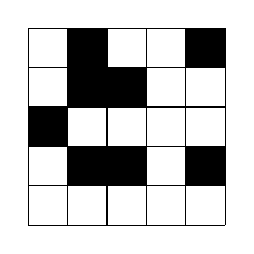
\begin{tikzpicture}[scale=0.5]
        \fill[black] (1,1) rectangle (2,2);
        \fill[black] (1,4) rectangle (2,5);
        \fill[black] (4,1) rectangle (5,2);
        \fill[black] (4,4) rectangle (5,5);
        \fill[black] (1,3) rectangle (2,4);
        \fill[black] (2,3) rectangle (3,4);
        \fill[black] (2,1) rectangle (3,2);
        \fill[black] (0,2) rectangle (1,3);
        \draw (0,0) grid (5,5);
    \end{tikzpicture}
\end{center}
contiene dos de estas subcuadrículas:
\begin{center}
    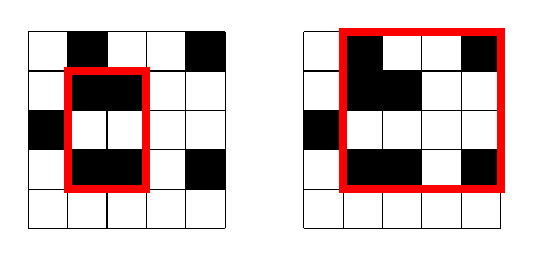
\begin{tikzpicture}[scale=0.5]
        \fill[black] (1,1) rectangle (2,2);
        \fill[black] (1,4) rectangle (2,5);
        \fill[black] (4,1) rectangle (5,2);
        \fill[black] (4,4) rectangle (5,5);
        \fill[black] (1,3) rectangle (2,4);
        \fill[black] (2,3) rectangle (3,4);
        \fill[black] (2,1) rectangle (3,2);
        \fill[black] (0,2) rectangle (1,3);
        \draw (0,0) grid (5,5);

        \fill[black] (7+1,1) rectangle (7+2,2);
        \fill[black] (7+1,4) rectangle (7+2,5);
        \fill[black] (7+4,1) rectangle (7+5,2);
        \fill[black] (7+4,4) rectangle (7+5,5);
        \fill[black] (7+1,3) rectangle (7+2,4);
        \fill[black] (7+2,3) rectangle (7+3,4);
        \fill[black] (7+2,1) rectangle (7+3,2);
        \fill[black] (7+0,2) rectangle (7+1,3);
        \draw (7+0,0) grid (7+5,5);

        \draw[color=red,line width=1mm] (1,1) rectangle (3,4);
        \draw[color=red,line width=1mm] (7+1,1) rectangle (7+5,5);
    \end{tikzpicture}
\end{center}

Existe un algoritmo de tiempo $O(n^3)$ para resolver el problema:
recorre todos los $O(n^2)$ pares de filas y para cada par
$(a, b)$ calcula el número de columnas que contienen un cuadrado negro
en ambas filas en tiempo $O(n)$.
El siguiente código asume que $\texttt{color}[y][x]$
denota el color en la fila $y$ y columna $x$:
\begin{lstlisting}
int conteo = 0;
for (int i = 0; i < n; i++) {
    if (color[a][i] == 1 && color[b][i] == 1) conteo++;
}
\end{lstlisting}
Entonces, esas columnas
representan $\texttt{conteo}(\texttt{conteo}-1)\div2$ subcuadrículas con esquinas negras,
porque podemos elegir cualquiera de los dos para formar una subcuadrícula.

Para optimizar este algoritmo, dividimos la cuadrícula en bloques
de columnas de tal manera que cada bloque consta de $N$
columnas consecutivas. Luego, cada fila se almacena como
una lista de números de $N$ bits que describen los colores
de los cuadrados. Ahora podemos procesar $N$ columnas al mismo tiempo
usando operaciones de bits. En el siguiente código,
$\texttt{color}[y][k]$ representa
un bloque de $N$ colores como bits.
\begin{lstlisting}
int conteo = 0;
for (int i = 0; i <= n / N; i++) {
    conteo += __builtin_popcount(color[a][i] & color[b][i]);
}
\end{lstlisting}
El algoritmo resultante funciona en tiempo $O(n^3/N)$.

Generamos una cuadrícula aleatoria de tamaño $2500 \times 2500$
y comparamos la implementación original y la optimizada con bits.
Mientras que el código original tardó $29,6$ segundos,
la versión optimizada con bits solo tardó $3,1$ segundos
con $N=32$ (números \texttt{int}) y $1,7$ segundos
con $N=64$ (números \texttt{long long}).

\section{Programación dinámica}

Las operaciones de bits proporcionan una forma eficiente y conveniente
de implementar algoritmos de programación dinámica
cuyos estados contienen subconjuntos de elementos,
porque tales estados se pueden almacenar como enteros.
A continuación, discutimos ejemplos de combinación
de operaciones de bits y programación dinámica.

\subsubsection{Selección óptima}

Como primer ejemplo, considera el siguiente problema:
Se nos dan los precios de $k$ productos
durante $n$ días, y queremos comprar cada producto
exactamente una vez.
Sin embargo, solo se nos permite comprar un producto como máximo
en un día.
¿Cuál es el precio total mínimo?
Por ejemplo, considera el siguiente escenario ($k=3$ y $n=8$):
\begin{center}
    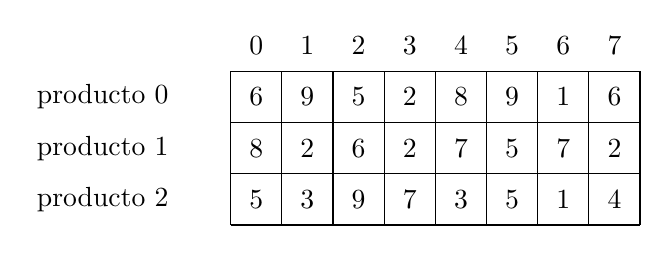
\begin{tikzpicture}[scale=.65]
        \draw (0, 0) grid (8,3);
        \node at (-2.5,2.5) {producto 0};
        \node at (-2.5,1.5) {producto 1};
        \node at (-2.5,0.5) {producto 2};

        \foreach \x in {0,...,7}
            {\node at (\x+0.5,3.5) {\x};}
        \foreach \x/\v in {0/6,1/9,2/5,3/2,4/8,5/9,6/1,7/6}
            {\node at (\x+0.5,2.5) {\v};}
        \foreach \x/\v in {0/8,1/2,2/6,3/2,4/7,5/5,6/7,7/2}
            {\node at (\x+0.5,1.5) {\v};}
        \foreach \x/\v in {0/5,1/3,2/9,3/7,4/3,5/5,6/1,7/4}
            {\node at (\x+0.5,0.5) {\v};}
    \end{tikzpicture}
\end{center}
En este escenario, el precio total mínimo es $5$:
\begin{center}
    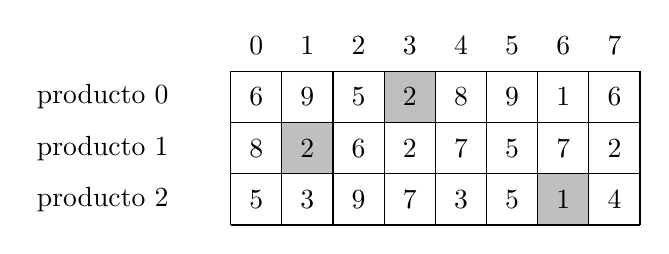
\begin{tikzpicture}[scale=.65]
        \fill [color=lightgray] (1, 1) rectangle (2, 2);
        \fill [color=lightgray] (3, 2) rectangle (4, 3);
        \fill [color=lightgray] (6, 0) rectangle (7, 1);
        \draw (0, 0) grid (8,3);
        \node at (-2.5,2.5) {producto 0};
        \node at (-2.5,1.5) {producto 1};
        \node at (-2.5,0.5) {producto 2};

        \foreach \x in {0,...,7}
            {\node at (\x+0.5,3.5) {\x};}
        \foreach \x/\v in {0/6,1/9,2/5,3/2,4/8,5/9,6/1,7/6}
            {\node at (\x+0.5,2.5) {\v};}
        \foreach \x/\v in {0/8,1/2,2/6,3/2,4/7,5/5,6/7,7/2}
            {\node at (\x+0.5,1.5) {\v};}
        \foreach \x/\v in {0/5,1/3,2/9,3/7,4/3,5/5,6/1,7/4}
            {\node at (\x+0.5,0.5) {\v};}
    \end{tikzpicture}
\end{center}

Definamos $\texttt{precio}[x][d]$ como el precio del producto $x$
en el día $d$.
Por ejemplo, en el escenario anterior $\texttt{precio}[2][3] = 7$.
Luego, que $\texttt{total}(S,d)$ denote el precio total mínimo
para comprar un subconjunto $S$ de productos en el día $d$.
Usando esta función, la solución al problema es
$\texttt{total}(\{0 \ldots k-1\},n-1)$.

Primero, $\texttt{total}(\emptyset,d) = 0$,
porque no cuesta nada comprar un conjunto vacío,
y $\texttt{total}(\{x\},0) = \texttt{precio}[x][0]$,
porque hay una forma de comprar un producto en el primer día.
Luego, se puede utilizar la siguiente recurrencia:
\begin{equation*}
    \begin{split}
        \texttt{total}(S,d) = \min( & \texttt{total}(S,d-1), \\
        & \min_{x \in S} (\texttt{total}(S \setminus x,d-1)+\texttt{precio}[x][d]))
    \end{split}
\end{equation*}
Esto significa que no compramos ningún producto en el día $d$
o compramos un producto $x$ que pertenece a $S$.
En este último caso, quitamos $x$ de $S$ y añadimos el
precio de $x$ al precio total.

El siguiente paso es calcular los valores de la función
usando programación dinámica.
Para almacenar los valores de la función, declaramos una matriz
\begin{lstlisting}
int total[1 << K][N];
\end{lstlisting}
donde $K$ y $N$ son constantes adecuadamente grandes.
La primera dimensión de la matriz corresponde a una representación de bits de un subconjunto.

Primero, los casos donde $d=0$ se pueden procesar de la siguiente manera:
\begin{lstlisting}
for (int x = 0; x < k; x++) {
    total[1 << x][0] = precio[x][0];
}
\end{lstlisting}
Luego, la recurrencia se traduce en el siguiente código:
\begin{lstlisting}
for (int d = 1; d < n; d++) {
    for (int s = 0; s < (1 << k); s++) {
        total[s][d] = total[s][d - 1];
        for (int x = 0; x < k; x++) {
            if (s & (1 << x)) {
                total[s][d] = min(total[s][d],
                                  total[s ^ (1<<x)][d - 1] + precio[x][d]);
            }
        }
    }
}
\end{lstlisting}
La complejidad temporal del algoritmo es $O(n 2^k k)$.

\subsubsection{De permutaciones a subconjuntos}

Usando programación dinámica, a menudo es posible
cambiar una iteración sobre permutaciones a
una iteración sobre subconjuntos.\footnote{Esta técnica fue introducida en 1962
    por M. Held y R. M. Karp \cite{hel62}.}
El beneficio de esto es que
$n!$, el número de permutaciones,
es mucho mayor que $2^n$, el número de subconjuntos.
Por ejemplo, si $n=20$, entonces
$n! \approx 2.4 \cdot 10^{18}$ y $2^n \approx 10^6$.
Así, para ciertos valores de $n$,
podemos recorrer eficientemente los subconjuntos pero no las permutaciones.

Como ejemplo, considera el siguiente problema:
Hay un ascensor con peso máximo $x$,
y $n$ personas con pesos conocidos
que quieren ir desde la planta baja
hasta la última planta.
¿Cuál es el número mínimo de viajes necesarios
si las personas entran al ascensor en un orden óptimo?

Por ejemplo, suponga que $x=10$, $n=5$
y los pesos son los siguientes:
\begin{center}
    \begin{tabular}{ll}
        persona & peso \\
        \hline
        0       & 2    \\
        1       & 3    \\
        2       & 3    \\
        3       & 5    \\
        4       & 6    \\
    \end{tabular}
\end{center}
En este caso, el número mínimo de viajes es 2.
Un orden óptimo es $\{0,2,3,1,4\}$,
que divide a las personas en dos viajes:
primero $\{0,2,3\}$ (peso total 10),
y luego $\{1,4\}$ (peso total 9).

El problema se puede resolver fácilmente en tiempo $O(n! n)$
probando todas las permutaciones de $n$ personas.
Sin embargo, podemos utilizar programación dinámica para obtener
un algoritmo más eficiente de $O(2^n n)$.
La idea es calcular para cada subconjunto de personas
dos valores: el número mínimo de viajes necesarios y
el peso mínimo de las personas que viajan en el último grupo.

Definamos $\texttt{peso}[p]$ como el peso de
la persona $p$.
Definimos dos funciones:
$\texttt{viajes}(S)$ es el número mínimo de
viajes para un subconjunto $S$,
y $\texttt{ultimo}(S)$ es el peso mínimo
del último viaje.
Por ejemplo, en el escenario anterior
\[ \texttt{viajes}(\{1,3,4\})=2 \hspace{10px} \textrm{y}
    \hspace{10px} \texttt{ultimo}(\{1,3,4\})=5,\]
porque los viajes óptimos son $\{1,4\}$ y $\{3\}$,
y el segundo viaje tiene un peso de 5.
Por supuesto, nuestro objetivo final es calcular el valor
de $\texttt{viajes}(\{0 \ldots n-1\})$.

Podemos calcular los valores
de las funciones de forma recursiva y luego aplicar
programación dinámica.
La idea es recorrer todas las personas
que pertenecen a $S$ y escoger de manera óptima
la última persona $p$ que entra en el ascensor.
Cada una de estas elecciones genera un subproblema
para un subconjunto más pequeño de personas.
Si $\texttt{ultimo}(S \setminus p)+\texttt{peso}[p] \le x$,
podemos agregar $p$ al último viaje.
De lo contrario, debemos reservar un nuevo viaje
que inicialmente solo contiene $p$.

Para implementar programación dinámica,
declaramos un arreglo
\begin{lstlisting}
pair<int, int> mejor[1 << N];
\end{lstlisting}
que contiene para cada subconjunto $S$
un par $(\texttt{viajes}(S),\texttt{ultimo}(S))$.
Establecemos el valor para un grupo vacío de la siguiente manera:
\begin{lstlisting}
mejor[0] = {1, 0};
\end{lstlisting}
Entonces, podemos llenar el arreglo de la siguiente manera:

\begin{lstlisting}
for (int s = 1; s < (1 << n); s++) {
    // valor inicial: se necesitan n + 1 viajes
    mejor[s] = {n + 1, 0};
    for (int p = 0; p < n; p++) {
        if (s & (1 << p)) {
            auto opción = mejor[s ^ (1 << p)];
            if (opción.second + peso[p] <= x) {
                // agregar p a un viaje existente
                opción.second += peso[p];
            } else {
                // reservar un nuevo viaje para p
                opción.first++;
                opción.second = peso[p];
            }
            mejor[s] = min(mejor[s], opción);
        }
    }
}
\end{lstlisting}
Ten en cuenta que el bucle anterior garantiza que
para cualquier dos subconjuntos $S_1$ y $S_2$
tal que $S_1 \subset S_2$, procesamos $S_1$ antes de $S_2$.
Por lo tanto, los valores de programación dinámica se calculan en el
orden correcto.

\subsubsection{Contar subconjuntos}

Nuestro último problema en este capítulo es el siguiente:
Sea $X=\{0 \ldots n-1\}$, y a cada subconjunto $S \subset X$
se le asigna un entero $\texttt{valor}[S]$.
Nuestra tarea es calcular para cada $S$
\[\texttt{suma}(S) = \sum_{A \subset S} \texttt{valor}[A],\]
es decir, la suma de los valores de los subconjuntos de $S$.

Por ejemplo, suponga que $n=3$ y los valores son los siguientes:
\begin{multicols}{2}
    \begin{itemize}
        \item $\texttt{valor}[\emptyset] = 3$
        \item $\texttt{valor}[\{0\}] = 1$
        \item $\texttt{valor}[\{1\}] = 4$
        \item $\texttt{valor}[\{0,1\}] = 5$
        \item $\texttt{valor}[\{2\}] = 5$
        \item $\texttt{valor}[\{0,2\}] = 1$
        \item $\texttt{valor}[\{1,2\}] = 3$
        \item $\texttt{valor}[\{0,1,2\}] = 3$
    \end{itemize}
\end{multicols}
En este caso, por ejemplo,
\begin{equation*}
    \begin{split}
        \texttt{suma}(\{0,2\}) &= \texttt{valor}[\emptyset]+\texttt{valor}[\{0\}]+\texttt{valor}[\{2\}]+\texttt{valor}[\{0,2\}] \\
        &= 3 + 1 + 5 + 1 = 10.
    \end{split}
\end{equation*}

Debido a que hay un total de $2^n$ subconjuntos,
una posible solución es recorrer todos
los pares de subconjuntos en tiempo $O(2^{2n})$.
Sin embargo, usando programación dinámica, podemos
resolver el problema en tiempo $O(2^n n)$.
La idea es centrarse en las sumas donde los
elementos que pueden eliminarse de $S$ están restringidos.

Denotemos a $\texttt{parcial}(S,k)$ como la suma de
valores de subconjuntos de $S$ con la restricción
de que solo los elementos $0 \ldots k$
pueden eliminarse de $S$.
Por ejemplo,
\[\texttt{parcial}(\{0,2\},1)=\texttt{valor}[\{2\}]+\texttt{valor}[\{0,2\}],\]
porque solo podemos eliminar elementos $0 \ldots 1$.
Podemos calcular valores de \texttt{suma} usando
valores de \texttt{parcial}, porque
\[\texttt{suma}(S) = \texttt{parcial}(S,n-1).\]
Los casos base para la función son
\[\texttt{parcial}(S,-1)=\texttt{valor}[S],\]
porque en este caso no se pueden eliminar elementos de $S$.
Luego, en el caso general, podemos usar la siguiente recurrencia:
\begin{equation*}
    \texttt{parcial}(S,k) = \begin{cases}
        \texttt{parcial}(S,k-1)                                           & k \notin S \\
        \texttt{parcial}(S,k-1) + \texttt{parcial}(S \setminus \{k\},k-1) & k \in S
    \end{cases}
\end{equation*}
Aquí nos centramos en el elemento $k$.
Si $k \in S$, tenemos dos opciones: podemos mantener $k$ en $S$
o eliminarlo de $S$.

Hay una forma especialmente ingeniosa de implementar el
cálculo de sumas. Podemos declarar un arreglo
\begin{lstlisting}
int suma[1 << N];
\end{lstlisting}
que contendrá la suma de cada subconjunto.
El arreglo se inicializa de la siguiente manera:
\begin{lstlisting}
for (int s = 0; s < (1<<n); s++) {
    suma[s] = valor[s];
}
\end{lstlisting}
Luego, podemos llenar el arreglo de la siguiente manera:
\begin{lstlisting}
for (int k = 0; k < n; k++) {
    for (int s = 0; s < (1 << n); s++) {
        if (s & (1 << k)) suma[s] += suma[s ^ (1 << k)];
    }
}
\end{lstlisting}
Este código calcula los valores de $\texttt{parcial}(S,k)$
para $k=0 \ldots n-1$ en el arreglo \texttt{suma}.
Dado que $\texttt{parcial}(S,k)$ siempre se basa en
$\texttt{parcial}(S,k-1)$, podemos reutilizar el arreglo
\texttt{suma}, lo que resulta en una implementación muy eficiente.

